


\begin{figure}
    \centering
    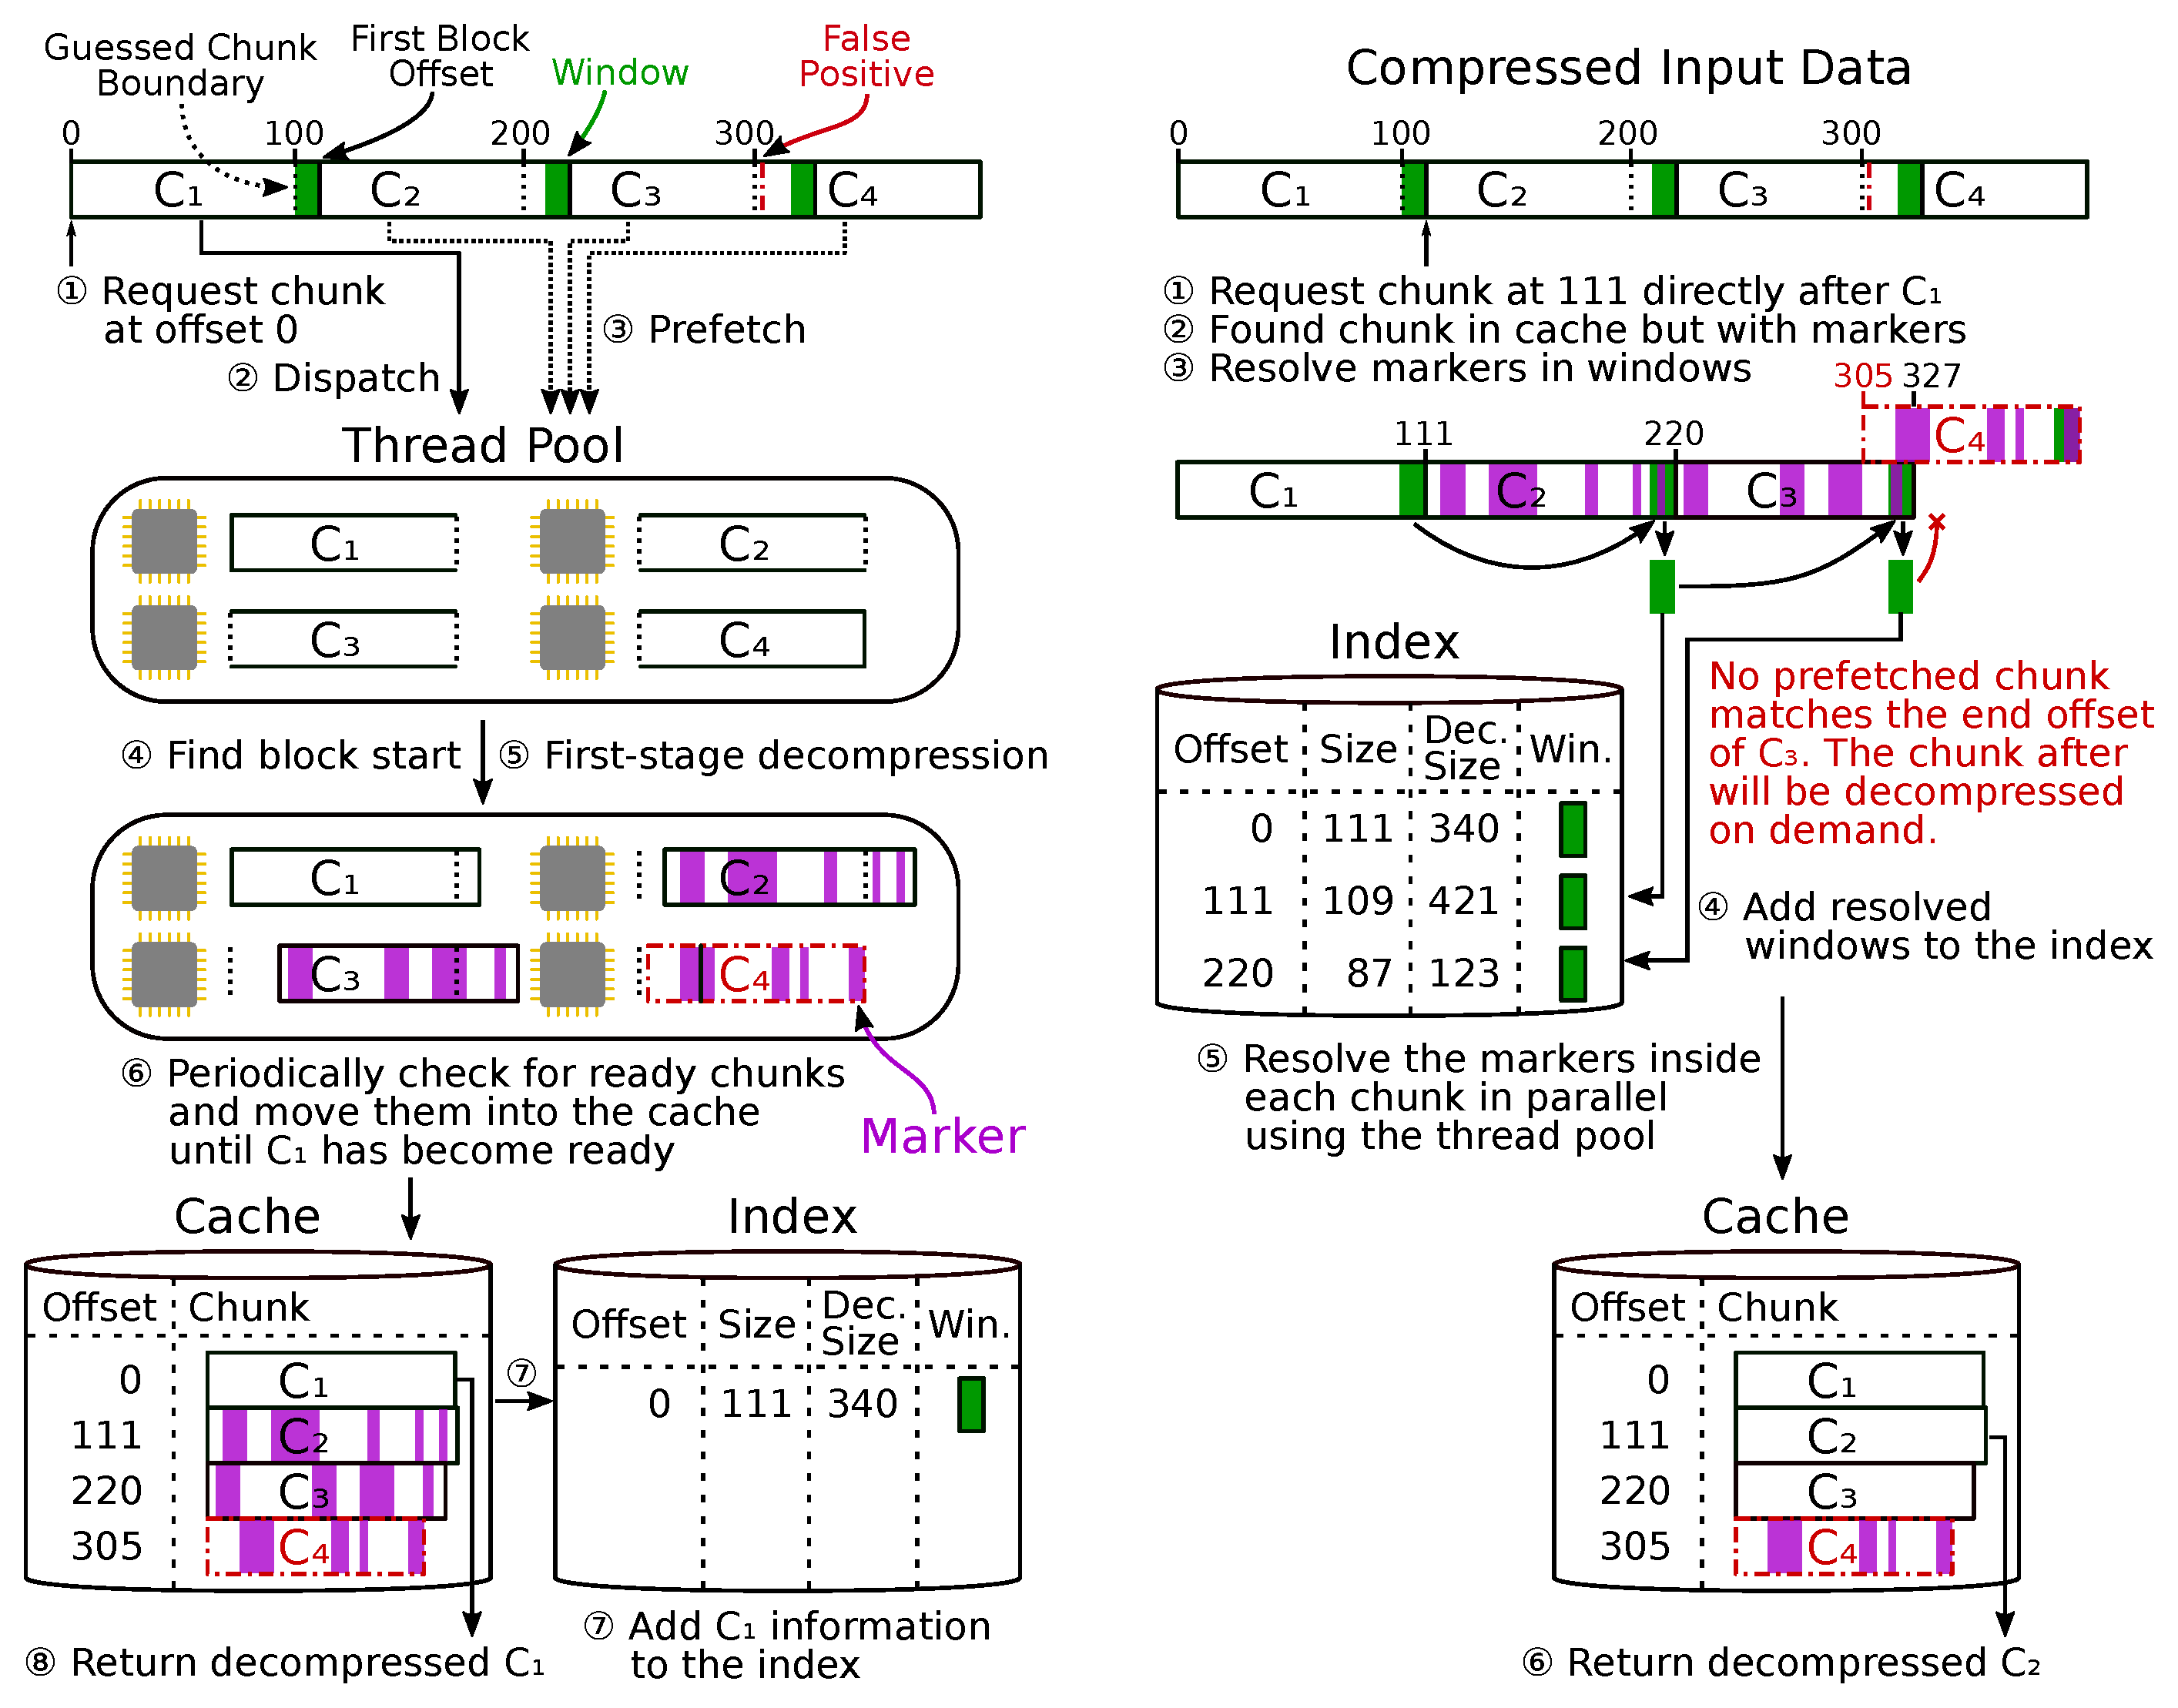
\includegraphics[width=\linewidth]{figures/cache-prefetch-architecture}
    \caption{Example of parallel decompression with the cache-and-prefetch architecture.
             Accessing the first chunk will prefetch further chunks in parallel.
             On access to the next chunk, the cached result can be used after the markers have been replaced.}
    \label{fig:parallel-decompression-process}
\end{figure}

\begin{figure}
    \centering
    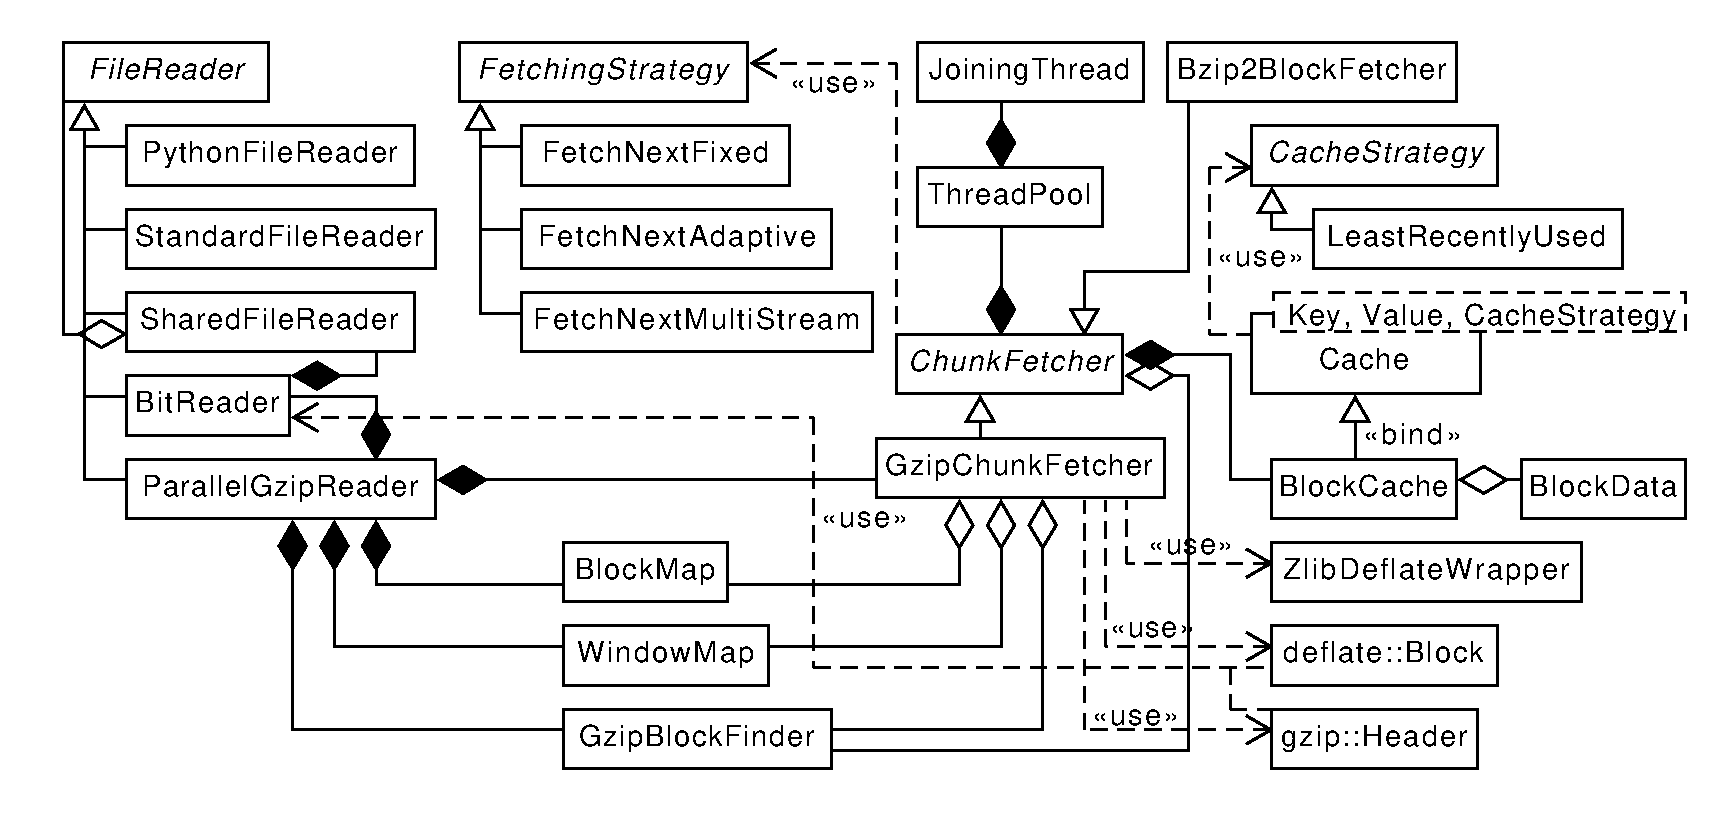
\includegraphics[width=\linewidth]{figures/class-diagram}
    \caption{Class diagram of the main components of our implementation.}
    \label{fig:architecture}
\end{figure}

\Cref{fig:architecture} shows the class hierarchy of \pragzip. The main components are:
\begin{itemize}
    \item A chunk fetcher that can opaquely prefetch and cache chunks in parallel
    \item A \blockfinder that returns likely \deflateblock offsets in a given data stream
    \item A gzip/deflate decoder that supports two-stage decoding
    \item A database containing \deflateblock offsets and sliding windows to start decoding from
\end{itemize}

The \texttt{FileReader} interface abstracts file access to support not only file access to regular files but also access to Python file-like objects.
A Python program can use this feature to implement recursive access to the contents of gzip-compressed gzip files. %
Our implementation fulfills the following design goals:
\begin{itemize}
    \item parallel chunk decompression
    \item only requires an initial decompression pass until the requested offset
    \item fast concurrent access at two different offsets
    \item seeking is possible in constant time when the requested offset exists in the index
    \item building the index is not a preprocessing step, it is done on the fly
    \item robust against false positives returned by the block finder
\end{itemize}
Concurrent access at different offsets is common when providing access to gzip-compressed (TAR) files via a user-space filesystem, e.g., provided by \CLITOOL{ratarmount}~\cite{ratarmount}.
Therefore, our implementation not only generalizes the approach from \pugz~\cite{pugz} to non-ASCII contents but also incorporates random access capabilities similar to \texttt{indexed\_gzip}~\cite{indexed_gzip}.

Robustness against false positives results from the cache acting as an intermediary with the offset as key.
When a thread finds a false positive, then the wrong result will be inserted into the cache with a wrong offset as key.
The main thread will request the next chunk based on the end offset of the previous chunk.
If the prefetching of the next chunk found a false positive, then the main thread will not be able to find any matching chunk in the cache and has to dispatch a new decompression task for the previous chunk's end offset.


\subsection{Seeking and Reading}

A seek only updates the internal position and the end-of-file flag.
Any further work for seeking will be done on the next read call.

\Cref{fig:parallel-decompression-process} shows an example of parallel decompression when reading consecutively from the start of the file.
During a read call to the \texttt{ParallelGzipReader} class, the internal \texttt{GzipChunkFetcher} is requested to return the chunk that contains the given position.
Access to a chunk triggers the prefetcher, even if the chunk has been found in the cache.
If the chunk has not been cached, then a decompression task is dispatched to the thread pool on demand.
Cached chunks can contain marker symbols.
Marker replacement is also dispatched to the thread pool.
At this point, all necessary information for a seek point in the index is available and will be inserted.
A fully decompressed chunk is returned to the caller after the marker replacement task has finished.


\subsection{Prefetching}

Prefetching is applied according to a prefetch strategy and is computed on the chunk indexes, not the chunk offsets.
The \chunkfetcher class combines a thread pool, a cache, a prefetch cache, a prefetching strategy, and a database for converting chunk offsets to and from chunk indexes.
The prefetch cache is separate from the cache of accessed chunks to avoid cache pollution of the latter cache caused by the prefetching.
For the common case of full file decompression, the access cache size is set to one and will only contain the last accessed chunk.
\Cref{fig:parallel-decompression-process} displays the two caches as one for brevity.

The current default prefetching strategy is an ad-hoc algorithm that works for concurrent sequential access to one or more files in a gzip-compressed TAR archive.
It is comparable to an exponentially incremented adaptive asynchronous multi-stream prefetcher~\cite{gill2007amp}.
The prefetch strategy returns the full degree of prefetch for the initial access so that decompression starts fully parallel.
The prefetch strategy does not keep track of previously prefetched chunks.
It returns a list of chunk indexes to prefetch based on the last accessed chunk indexes.
The prefetcher has to filter out already cached chunks and chunks that are currently being prefetched.


\subsection{Chunk Decompression}

The \texttt{GzipChunkFetcher} class extends the \chunkfetcher class with the seek point index.
The index contains compressed offsets, uncompressed offsets, and the \backrefwindow for each chunk.
The \texttt{Gzip\-Chunk\-Fetcher} also provides the implementation for the chunk decompression task that is dispatched to the thread pool.
If a \backrefwindow exists in the index for a chunk offset, then the decompression task will delegate decompression to zlib.
If no \backrefwindow exists, then the custom-written \pragzip gzip decompressor will try to decompress at candidate offsets returned by the \blockfinder until decompression succeeds.
The decompressor will stop when a \dynblock or \rawblock that starts at or after the given stop offset has been encountered.
This stop condition excludes \fixedblocks because the \blockfinder does not look for those.
If the stop condition does not match the \blockfinder search conditions, then performance will degrade because the prefetched subsequent chunk offset will not be found in the cache and therefore has to be decompressed again.

\Pragzip implements full gzip parsing consisting of: gzip header parsing, deflate block parsing, and gzip footer parsing.
For \deflate parsing, it supplies the \texttt{deflate::Block} class, which supports two-stage decompression as well as conventional decompression when a \backrefwindow is given.
For \rawblocks, it contains a fast path that simply copies the raw data into the result buffer.
The \deflate decompressor also keeps track of the last non-resolved marker symbol.
Decompression will fall back to the faster conventional decompression if there is no marker symbol in the \backrefwindow.
This improves performance when a file contains large \rawblocks and for data compressed with only few backward pointers.


\subsection{Block Finder}

The \blockfinder returns the next \deflateblock candidate offset when given an offset from which to start searching.
It may return false positives and should but is not required to find all valid \deflate blocks.

False positives cannot be avoided when searching from an arbitrary offset.
When compressing a non-compressible gzip-file with gzip, the resulting gzip stream will consist of \rawblocks.
The verbatim parts of those blocks contain valid \deflate blocks of the gzip file that has been compressed.
These can be detected as false positives during parallel decompression.

The \blockfinder is split into specialized \deflateblock finders for \dynblocks and \rawblocks.
These two are combined by finding candidates for both and subsequently returning the result with the lower offset.


\subsubsection{Non-Compressed Blocks}

The \blockfinder for \rawblocks looks for a pair of 16-bit length and 16-bit bit-wise negated length contained in the header as illustrated in \cref{fig:deflate_blocks}.
The false positive rate for this check by itself is once every $2^{16}\SI{}{\byte} = \SI{64}{\kibi\byte}$ because the length is byte-aligned and can be of any length including $0$, which leaves the 16-bit bit-wise negated length to be checked.

The false positive rate is further reduced by also checking the block type, requiring the final-block bit to be 0, and requiring the padding to achieve byte-alignment to be filled with zeros.
Gzip compressed files with non-zero padding were not encountered.
Applying the \rawblock finder on 12 samples of \SI{1}{\gibi\byte} of random data, yields \SI{2040(90)}{} false positives on average, i.e., once every \SI{514(23)}{\kibi\byte} specified with one standard deviation.

In comparison to the \dynblock finder described in \cref{sct:dynblocks}, the false positive rate is higher.
But, this does not slow down overall performance because decompression of \rawblocks consists of a fast \texttt{memcpy} followed by a check of the next block header, which is likely to fail for a false positive.
Searching for \rawblocks is $7\times$ faster than the \blockfinder for \dynblocks, see \cref{fig:components-benchmarks} in \cref{sct:evaluation}.

Care has to be taken when matching the requested bit offset with the block found by the \rawblock finder.
Bit offsets of \rawblocks can be ambiguous because the length of the zero-padding is not known.
The preceding bits for the block type and the non-final bit are also zero and thus indistinguishable from the zero-padding.


\subsubsection{Compressed with Dynamic Huffman Codes}
\label{sct:dynblocks}

Finding \dynblocks is a bottleneck of the decoder because most \deflate blocks contain dynamic Huffman codes.
Checking these for correctness is more computationally intensive than for \rawblocks.
The steps for checking a \dynblock for correctness are in order:

\begin{enumerate}
    \item The final-block bit must be 0
    \item The two block-type bits must be ${01}_2$
    \item The five bits containing the number of literal/length codes must not be 30 or 31
    \item The \precode bit triplets must represent a valid and efficient \huffcode
    \item The data decoded with the \precode must not contain invalid backward pointers
    \item The Distance \huffcode must be valid and efficient
    \item The Literal \huffcode must be valid and efficient
\end{enumerate}

If any of these steps fail for a given offset, then that offset is filtered and the next offset will be tested.

\begin{figure}
    \centering
    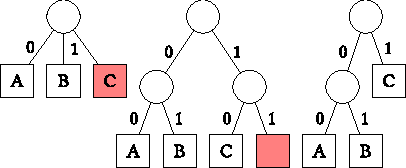
\includegraphics[scale=1]{figures/huffman-trees}
    \caption{
        Three Huffman codes with invalid tree nodes highlighted in red.
        The code lengths for A, B, C are respectively given as (left) 1,1,1, (middle) 2,2,2, (right) 2,2,1.
        \textbf{Left:} The third symbol of bit length 1 is invalid because only two symbols can be encoded with a single bit.
        \textbf{Middle:} The code is inefficient because the Huffman code 11 is unused.
        \textbf{Right:} The code is valid. All available leaf nodes are used.
    }
    \label{fig:huffman-check}
\end{figure}

Huffman codes are stored as a list of code lengths per symbol.
Huffman codes will be invalid if there are more symbols with a given code length than the binary tree permits.
Huffman codes are not efficient if there are unused leaves in the binary tree.
\Cref{fig:huffman-check} illustrates the requirements on the Huffman code.



\begin{table}[htp]
    \centering
    \begin{tabular}{l|S[table-format=6.3(4)e2, separate-uncertainty]}
        Tested bit positions         & 1e12 \\
        \hline
        Invalid final block          & 500000.1(7)e6 \\
        Invalid compression type     & 375000.0(4)e6 \\
        Invalid \precode size         & 7812.47(14)e6 \\
        Invalid \precode code         & 77451.6(6)e6 \\
        Non-optimal \precode code     & 39256.9(4)e6 \\
        \hline
        Invalid \precode-encoded data & 386.66(5)e6 \\
        Invalid distance code        & 14.291(6)e6 \\
        Non-optimal distance code    & 77.126(16)e6 \\
        \hline
        Invalid literal code         & 340.6(10)e3 \\
        Non-optimal literal code     & 517.2(14)e3 \\
        \hline
        \hline
        Valid \deflate headers        & 202(27) \\
    \end{tabular}
    \caption{%
        Empirical filter frequencies listed top-down in the order they are checked.
        To get these frequencies, the \dynblock finder has been applied to \SI{1}{\tera\bit} + \SI{2300}{\bit} of data.
        It was chosen such that it can accommodate \SI{1e12} test positions that all have sufficient bits for the maximum possible \deflate header size.
        This simulation has been repeated \num{12} times.
        The uncertainties are specified with one standard deviation.
    }
    \label{tab:false_positives}
\end{table}

\Cref{tab:false_positives} shows empirical results for the amount of filtering for each of these checks.
It shows the importance of filtering as early as possible.

A lookup cache is used to speed up the first three checks.
Currently, this cache looks up a 14-bit value and returns an 8-bit number representing the offset of a potential \dynblock.
If 0 is returned, the \precode bits will be checked next.

Seeking inside the bit stream is computationally expensive if it requires refilling the internal buffer.
A 14-bit large buffer for the lookup table and a 61-bit large buffer for the \precode are maintained to reduce seeking.
The \precode check itself has also been optimized to filter as soon as the symbol length frequencies have been calculated.
It uses lookup tables and bit-level parallelism to speed up the computation of the frequency histograms.

Consider this example of adding two independent numbers, each packed into four bits, using only a single 8-bit addition instead of two separate 4-bit additions:
\begin{equation*}
    0101\,1101_2 + 0001\,0001_2 = 0110\,1110_2
\end{equation*}
The addition of the two 4-bit numbers in the high bits on the left is independent of the low bits if and only if the sum of the two 4-bit numbers in the lower bits does not overflow the range that can be represented with 4 bits.

The frequency histogram uses 5 bits per frequency, which is sufficient to avoid overflows because there are only up to 19 \precode symbols.
This is a total of 40 bits because there are 8 different code lengths from 0 to 7.
This bit packing also enables the usage of another lookup table for testing the histogram validity.
This table takes 20 consecutive bits corresponding to the frequencies for code lengths 1 to 5 as input.

This is followed by a short loop to filter all invalid or non-optimal \huffcodes, see \cref{fig:huffman-check}.
All lookup tables are computed at compile-time by making frequent use of the extended C++17 \texttt{constexpr} keyword support.
After this lookup table check is passed, the \huffcode structure for the \precode has to be created in a separate step.
This is partly duplicated work but it is only done in the unlikely case that the checks succeed.
We also found that only 1526 \precode frequency histograms belong to valid Huffman codes.
We precalculated this list of valid histograms in an attempt to reduce the histogram validity check to a simple lookup.
This did not improve performance.

The \huffcodes for the \deflate literals and distance codes are only initialized after both were found to be valid in order to speed up the preemptive filtering further.
This also leads to some duplicate work if both \huffcodes are valid, which, as shown in \cref{tab:false_positives}, only happens once in 5 billion.
See \cref{sct:evaluation} for a comparison of the effect of these optimizations.


\subsubsection{Compressed with Fixed Huffman Codes}

The implemented \blockfinder does not try to find \fixedblocks because only the final-block bit and the two block type bits can be checked without starting the decompression.
Further checks on the length or contents of the decompressed stream could be imposed but those would make assumptions that are not valid for all gzip-compressed files.
Fortunately, these types of blocks are rare and in practice only used for very small files or end-of-stream blocks that contain only a few bytes of data.
In the worst case of a gzip file only containing \fixedblocks, this would result in only one thread decompressing the file while the others threads try and fail to find valid blocks.


\subsubsection{Blocked GNU Zip Format}

The Blocked GNU Zip Format (BGZF)~\cite{htslib} splits the data into fixed-size streams and uses the gzip extra field~\cite{RFC1952} to store the decompressed stream size.
This makes it trivial to gather \deflateblock offsets to start parallel decompression from.
Furthermore, such start offsets do not require the decoded data from the previous blocks.
Because of this, the two-stage decoding can be skipped and parallel BGZF file decompression is trivial.
The \texttt{GzipChunkFetcher} contains specialized fast paths if a BGZF file has been detected.
